\cleardoublepage
\chapter{Desain dan Implementasi}
\label{chap:desain-konsep-solusi}

% Catatan: bab ini menggunakan TikZ (shapes, arrows.meta, positioning, calc),
% pgfplots (compat=1.17), booktabs, dan listings. Pastikan paket-paket tersebut
% sudah dimuat pada preamble dokumen utama (main.tex).

Bab III telah menurunkan kebutuhan fungsional (KF-01 sampai KF-12) dan kebutuhan
nonfungsional (KNF-01 sampai KNF-08) ADADeH, serta menetapkan CNN pada
mel-spectrogram (alternatif A2) sebagai pendekatan deteksi yang dipilih melalui
matriks keputusan pada Subbab III.3. Bab ini menerjemahkan kebutuhan dan pilihan
tersebut menjadi rancangan yang konkret dan menjabarkan purwarupa yang telah
diimplementasikan secara nyata sebagai aplikasi web ADADeH berbasis Streamlit.
Subbab \ref{sec:desain-sistem} menguraikan desain sistem secara keseluruhan,
yaitu bagaimana kebutuhan diwujudkan menjadi alur kerja dan keluaran yang
diterima pengguna. Subbab \ref{sec:arsitektur-sistem} menjabarkan arsitektur
sistem, mulai dari pembagian peran klien dan server, susunan paket perangkat
lunak \texttt{adadeh} yang menjalankan setiap tahap pemrosesan, hingga susunan
lapisan model klasifikasi. Subbab \ref{sec:implementasi} menyajikan implementasi
purwarupa secara lengkap, yaitu (a) pengembangan model pada notebook: akuisisi
data, pra-pemrosesan audio, pembangunan model CNN, pelatihan, dan evaluasi awal;
serta (b) pembangunan aplikasi: validasi dan dekode audio yang diperkuat dari
sisi keamanan, pemuatan model dengan verifikasi integritas, pemeriksaan mutu
rekaman, orkestrasi layanan dan antarmuka pengguna, serta evaluasi purwarupa
yang mereproduksi baseline notebook sekaligus melengkapi metrik Equal Error Rate
(EER) yang sebelumnya belum dihitung. Seluruh uraian mengacu langsung pada
notebook pengembangan ADADeH dan kode sumber paket \texttt{adadeh} pada aplikasi
yang telah dibangun.

\section{Desain Sistem}
\label{sec:desain-sistem}

\subsection{Prinsip Desain}
\label{subsec:prinsip-desain}

Tiga prinsip mendasari desain ADADeH, yang masing-masing diturunkan langsung dari
kebutuhan sistem pada Bab III.

\begin{enumerate}
  \item \textbf{Pipeline otomatis end-to-end.} Sejak rekaman diunggah hingga label
  dan skor keyakinan ditampilkan, seluruh tahap (KF-02 sampai KF-08) berjalan
  berurutan tanpa intervensi manual, memenuhi kriteria keberhasilan kedua pada
  Bab I.
  \item \textbf{Konsistensi parameter latih dan infer.} Parameter pra-pemrosesan
  (\textit{sampling rate}, durasi potongan, jumlah \textit{mel bin}) serta statistik
  normalisasi dan ambang keputusan yang digunakan saat prediksi harus identik
  dengan yang digunakan saat pelatihan. Prinsip ini menjawab KNF-08 dan konsekuensi
  teknis yang telah ditekankan pada Subsubbab II.1.2.2, yaitu bahwa model akan salah
  membaca data apabila skala masukannya berubah.
  \item \textbf{Pemisahan tanggung jawab antarmuka dan pemrosesan.} Mengikuti
  arsitektur klien--server pada Subbab II.3.3, peramban pengguna hanya bertanggung
  jawab menerima masukan dan menampilkan keluaran, sedangkan seluruh pemrosesan
  audio dan inferensi model berjalan di sisi server. Pemisahan ini memudahkan
  pengguna awam (KP-01, KP-03) dan menjaga agar perangkat pengguna tidak perlu
  memenuhi spesifikasi komputasi tertentu (Subsubbab II.3.1.3).
\end{enumerate}

\subsection{Alur Proses Sistem}
\label{subsec:alur-proses-sistem}

Alur proses ADADeH terdiri atas delapan tahap yang mengalir dari masukan rekaman
hingga keluaran hasil deteksi. Gambar \ref{fig:alur-proses} mengilustrasikan alur
tersebut, sedangkan Tabel \ref{tab:pemetaan-alur-kf} memetakan setiap tahap kepada
kebutuhan fungsional yang dipenuhinya.

\begin{figure}[htbp]
  \centering
  \begin{tikzpicture}[
      font=\small,
      node distance=6mm and 8mm,
      proc/.style={rectangle, rounded corners, draw=black, thick,
        minimum width=2.6cm, minimum height=1.05cm, align=center,
        fill=gray!8},
      decide/.style={diamond, draw=black, thick, aspect=2.2,
        minimum width=2.2cm, minimum height=1cm, align=center, fill=gray!15},
      term/.style={rectangle, rounded corners=3mm, draw=black, thick,
        minimum width=2.2cm, minimum height=0.9cm, align=center, fill=white},
      arrow/.style={-{Latex[length=2.2mm]}, thick}
    ]
    \node[term] (mulai) {Pengguna\\mengunggah rekaman};
    \node[proc, right=of mulai] (validasi) {Validasi \&\\dekode berkas};
    \node[decide, right=of validasi] (lolos) {Berkas\\valid?};
    \node[proc, above right=4mm and 9mm of lolos] (tolak) {Tampilkan\\pesan kesalahan};
    \node[proc, below=of validasi, yshift=-4mm] (seragam) {Resampling \&\\mono-kanal};
    \node[proc, right=of seragam] (potong) {Pemotongan\\menjadi $K$ potongan};
    \node[proc, right=of potong] (mel) {Ekstraksi\\mel-spectrogram};
    \node[proc, below=of mel, yshift=-4mm] (norm) {Normalisasi\\($\mu,\sigma$ data latih)};
    \node[proc, left=of norm] (cnn) {Inferensi CNN\\per potongan};
    \node[proc, left=of cnn] (agregasi) {Agregasi skor\\$\bar{p}$ (Pers.~III.2)};
    \node[proc, below=of agregasi, yshift=-4mm] (label) {Penentuan label\\\& skor keyakinan};
    \node[term, right=of label] (tampil) {Tampilkan hasil\\\& batasan};
    \node[proc, right=of tampil] (hapus) {Hapus berkas\\\& data antara};

    \draw[arrow] (mulai) -- (validasi);
    \draw[arrow] (validasi) -- (lolos);
    \draw[arrow] (lolos) -- node[above,font=\scriptsize]{tidak} (tolak);
    \draw[arrow] (lolos) -- node[left,font=\scriptsize]{ya} (seragam);
    \draw[arrow] (seragam) -- (potong);
    \draw[arrow] (potong) -- (mel);
    \draw[arrow] (mel) -- (norm);
    \draw[arrow] (norm) -- (cnn);
    \draw[arrow] (cnn) -- (agregasi);
    \draw[arrow] (agregasi) -- (label);
    \draw[arrow] (label) -- (tampil);
    \draw[arrow] (tampil) -- (hapus);
  \end{tikzpicture}
  \caption{Alur Proses Sistem ADADeH dari Unggahan hingga Penyajian Hasil}
  \label{fig:alur-proses}
\end{figure}

\begin{table}[htbp]
  \centering
  \caption{Pemetaan Tahap Alur Proses terhadap Kebutuhan Fungsional}
  \label{tab:pemetaan-alur-kf}
  \begin{tabular}{@{}cll@{}}
    \toprule
    \textbf{Tahap} & \textbf{Deskripsi} & \textbf{KF Terkait} \\
    \midrule
    1 & Validasi ukuran, durasi, dan dekode berkas & KF-02 \\
    2 & Resampling ke \textit{sampling rate} data latih, penyeragaman kanal & KF-03 \\
    3 & Pemotongan rekaman menjadi $K$ potongan tetap & KF-04 \\
    4 & Ekstraksi mel-spectrogram skala dB per potongan & KF-05 \\
    5 & Normalisasi menggunakan statistik data latih & KF-05, KNF-08 \\
    6 & Inferensi skor deepfake $p_k$ per potongan oleh CNN & KF-06 \\
    7 & Agregasi skor $\bar{p}$ dan penentuan label dengan ambang $\tau$ & KF-07 \\
    8 & Penyajian label, skor keyakinan, dan keterangan batasan & KF-08, KF-09, KF-10 \\
    \bottomrule
  \end{tabular}
\end{table}

Tahap 1 sampai 7 berjalan otomatis tanpa keterlibatan pengguna, sesuai prinsip
pipeline \textit{end-to-end} pada Subsubbab \ref{subsec:prinsip-desain}. Apabila
validasi pada tahap 1 tidak lolos, misalnya berkas bukan audio atau berukuran
melebihi batas KNF-03, sistem langsung menampilkan pesan kesalahan tanpa
melanjutkan ke tahap berikutnya. Jika rekaman lolos validasi namun menunjukkan
indikasi mutu rendah (durasi terlalu singkat, dominan hening, atau \textit{clipping}),
peringatan tersebut ditampilkan bersamaan dengan label pada tahap 8, bukan sebagai
penolakan, karena hal ini memenuhi KF-10 sekaligus tetap memberikan indikasi awal
kepada pengguna sesuai KP-07. Setelah hasil ditampilkan dan sesi pengguna berakhir,
berkas unggahan serta data antara (waveform dan mel-spectrogram sementara) dihapus
untuk memenuhi KF-12 dan KNF-05.

\subsection{Rancangan Keluaran bagi Pengguna}
\label{subsec:rancangan-keluaran}

Mengingat pengguna sasaran adalah pengguna awam dan pendamping pelaporan
(Subsubbab III.2.1), keluaran ADADeH dirancang dalam bahasa yang sederhana namun
tetap menyertakan keterangan yang diperlukan untuk penggunaan hasilnya sebagai
indikasi awal. Tabel \ref{tab:elemen-keluaran} merinci setiap elemen keluaran.

\begin{table}[htbp]
  \centering
  \caption{Elemen Keluaran ADADeH bagi Pengguna}
  \label{tab:elemen-keluaran}
  \begin{tabular}{@{}p{3.1cm}p{7.6cm}l@{}}
    \toprule
    \textbf{Elemen} & \textbf{Isi} & \textbf{KF/KP Terkait} \\
    \midrule
    Label & ``Terindikasi asli'' atau ``Terindikasi deepfake'' & KF-08, KP-03 \\
    Skor keyakinan & Nilai $c=\max(\bar{p},1-\bar{p})$ dalam persen & KF-08, KP-03 \\
    Keterangan batasan & Penegasan bahwa hasil bersifat indikasi awal, dilatih pada satu
    dataset berbahasa Inggris, dan bukan pengganti pemeriksaan forensik digital & KF-09,
    KP-04 \\
    Peringatan mutu & Catatan apabila rekaman terlalu singkat, dominan hening, atau
    terindikasi \textit{clipping} & KF-10, KP-07 \\
    Ringkasan terunduh & Nama berkas, durasi, waktu pemeriksaan, nilai \textit{hash}
    SHA-256, label, skor, versi model, dan keterangan batasan & KF-11, KP-09 \\
    \bottomrule
  \end{tabular}
\end{table}

Urutan penyajian mengikuti pedoman interaksi manusia--AI pada Subsubbab III.2.2
(KP-03): label dan skor ditampilkan paling menonjol, diikuti keterangan batasan dan
peringatan mutu, dan ringkasan terunduh disediakan sebagai opsi tambahan bagi
pendamping pelaporan. Dengan rancangan ini, desain sistem pada subbab ini telah
mencakup seluruh kebutuhan fungsional KF-01 sampai KF-12 dan menjadi acuan langsung
bagi arsitektur pada Subbab \ref{sec:arsitektur-sistem}.

\section{Arsitektur Sistem}
\label{sec:arsitektur-sistem}

\subsection{Arsitektur Klien--Server}
\label{subsec:arsitektur-klien-server}

Mengikuti pilihan platform Streamlit pada Subbab II.3.2.5 dan II.3.3, ADADeH
diimplementasikan dengan arsitektur klien--server dua lapis: peramban pengguna
sebagai klien, dan aplikasi Python (\texttt{streamlit\_app.py}, menjalankan
paket \texttt{adadeh}) sebagai server yang menjalankan seluruh pemrosesan audio
dan inferensi model. Pada tahap purwarupa saat ini, klien dan server berjalan
pada komputer yang sama (\textit{localhost}); pembagian peran tetap mengikuti
pola klien--server penuh agar aplikasi dapat dipindahkan ke penempatan jaringan
tanpa mengubah struktur kode. Gambar \ref{fig:arsitektur-klien-server}
menggambarkan pembagian komponen tersebut beserta protokol komunikasi yang
menghubungkannya, sejalan dengan Tabel II.4.

\begin{figure}[htbp]
  \centering
  \begin{tikzpicture}[
      font=\small,
      box/.style={rectangle, draw=black, thick, rounded corners,
        minimum height=1cm, align=center, inner sep=2.5mm},
      sub/.style={rectangle, draw=black, minimum width=4.6cm,
        minimum height=0.95cm, align=center, fill=gray!8, inner sep=1.5mm},
      arrow/.style={-{Latex[length=2.2mm]}, thick}
    ]
    \node[box, fill=blue!6, minimum width=3.2cm] (klien) at (0,0)
      {\textbf{Klien}\\Peramban pengguna\\(antarmuka Streamlit)};

    \node[box, fill=orange!8, minimum width=6cm, minimum height=5.8cm]
      (server) at (6.7,0) {};
    \node[font=\small\bfseries] at (6.7,2.85) {Server};
    \node[sub] (modul1) at (6.7,1.75) {\texttt{audio.py} + \texttt{quality.py}\\validasi, dekode \& mutu};
    \node[sub] (modul2) at (6.7,0) {\texttt{preprocessing.py}\\ekstraksi mel-spectrogram};
    \node[sub] (modul3) at (6.7,-1.75) {\texttt{model.py} + \texttt{contracts.py}\\inferensi CNN \& integritas};

    \node[box, fill=green!10, minimum width=4.4cm, minimum height=1cm]
      (artefak) at (6.7,-5.2) {Artefak model\\(terverifikasi SHA-256)};

    \draw[arrow] ($(klien.east)+(0,0.3)$) -- ++(0.55,0) |-
      (modul1.west);
    \node[font=\scriptsize, align=center] at (3.8,1.0) {HTTPS\\(unggah berkas)};

    \draw[arrow] ($(modul2.west)+(0,-0.35)$) -- ++(-2.65,0) |-
      ($(klien.east)+(0,-0.3)$);
    \node[font=\scriptsize, align=center] at (3.8,-1.0) {WSS\\(status \& hasil)};

    \draw[arrow] (modul3.south) -- ++(0,-0.75) -| (artefak.north);
    \node[font=\scriptsize, align=center] at (8.9,-3.4) {memuat bobot \&\\konfigurasi};
  \end{tikzpicture}
  \caption{Arsitektur Klien--Server ADADeH}
  \label{fig:arsitektur-klien-server}
\end{figure}

Peran masing-masing komponen adalah sebagai berikut.

\begin{enumerate}
  \item \textbf{Klien.} Peramban menampilkan halaman unggah, indikator kemajuan, dan
  hasil akhir. Klien tidak menyimpan maupun mengolah rekaman; seluruh berkas yang
  dipilih pengguna melalui \texttt{st.file\_uploader} segera dikirim ke server
  melalui HTTP/HTTPS (Subbab II.3.4), sedangkan pembaruan tampilan selama
  pemrosesan berlangsung disalurkan melalui WebSocket/WSS (Subbab II.3.5).
  \item \textbf{Modul validasi, dekode, dan pemeriksaan mutu
  (\texttt{audio.py}, \texttt{quality.py}).} Modul ini menjalankan Tahap 1
  sampai 3 pada Gambar \ref{fig:alur-proses} sekaligus memperkuatnya dari sisi
  keamanan: dekode berkas dijalankan pada proses terpisah (\textit{subprocess})
  berbatas waktu, berkas M4A/ISO-BMFF diperiksa secara khusus agar tidak berisi
  rujukan data eksternal, dan rekaman yang lolos dekode diperiksa mutunya
  (hening, \textit{clipping}, durasi) sebelum dilanjutkan ke tahap ekstraksi
  fitur. Rincian keduanya dibahas pada Subsubbab \ref{subsec:implementasi-audio}
  dan \ref{subsec:implementasi-mutu}.
  \item \textbf{Modul ekstraksi mel-spectrogram (\texttt{preprocessing.py}).}
  Modul ini menjalankan Tahap 4 dan 5, membentuk mel-spectrogram skala dB dan
  menormalisasinya dengan statistik data latih yang tersimpan pada artefak
  konfigurasi.
  \item \textbf{Modul inferensi dan integritas model (\texttt{model.py},
  \texttt{contracts.py}).} Modul ini memuat bobot model terlatih, memverifikasi
  integritasnya (lihat butir Artefak model), dan menjalankan Tahap 6 dan 7,
  yaitu menghitung skor per potongan serta mengagregasinya menjadi skor dan
  label akhir melalui \texttt{prediction.py}.
  \item \textbf{Artefak model.} Berkas \texttt{adadeh\_cnn.keras} menyimpan
  arsitektur dan bobot CNN, sedangkan \texttt{meta.json} menyimpan seluruh
  parameter pra-pemrosesan, statistik normalisasi, dan ambang keputusan yang
  digunakan selama pelatihan (dibahas lebih lanjut pada Subsubbab
  \ref{subsec:arsitektur-konfigurasi}). Keduanya dimuat bersama oleh server saat
  aplikasi dijalankan, sehingga parameter pelatihan dan inferensi selalu konsisten
  (KNF-08). Sebelum dimuat, nilai \textit{hash} SHA-256 kedua berkas diverifikasi
  terhadap nilai yang tertanam pada kode aplikasi; apabila tidak cocok, aplikasi
  menghentikan pemuatan tanpa cadangan (\textit{fallback}) apa pun, untuk mencegah
  model yang rusak atau telah diubah dipakai tanpa disadari (Subsubbab
  \ref{subsec:implementasi-model-runtime}).
  \item \textbf{Modul orkestrasi, antarmuka, dan pelaporan (\texttt{service.py},
  \texttt{ui.py}, \texttt{reporting.py}).} Modul ini menghubungkan seluruh modul
  di atas menjadi satu alur \texttt{analyze\_audio()}, menyajikannya pada
  antarmuka Streamlit (\texttt{st.file\_uploader}, \texttt{st.status}), dan
  menyediakan ringkasan hasil yang dapat diunduh dalam format JSON maupun teks
  (Subsubbab \ref{subsec:implementasi-layanan}).
\end{enumerate}

\subsection{Arsitektur Paket Perangkat Lunak \texttt{adadeh}}
\label{subsec:arsitektur-modul-pemrosesan}

Seluruh modul server pada Gambar \ref{fig:arsitektur-klien-server} diwujudkan
sebagai satu paket Python terinstal bernama \texttt{adadeh} (struktur
\texttt{src}, didefinisikan melalui \texttt{pyproject.toml}), bukan sebagai
satu berkas tunggal. Pemisahan ini memudahkan setiap tanggung jawab diuji
secara independen (unit, integrasi, kesetaraan terhadap notebook, dan
antarmuka -- Subsubbab \ref{subsec:implementasi-pengujian}) serta memudahkan
penelusuran kesalahan. Tabel \ref{tab:modul-pemrosesan} merinci sembilan modul
penyusun paket tersebut, tanggung jawabnya, dan kebutuhan fungsional/nonfungsional
yang dipenuhinya; urutannya sejalan dengan alur data pada Gambar
\ref{fig:alur-proses}, dari dekode berkas hingga penyajian serta pembersihan
hasil.

\begin{table}[htbp]
  \centering
  \caption{Modul Penyusun Paket \texttt{adadeh}}
  \label{tab:modul-pemrosesan}
  \begin{tabular}{@{}p{3.1cm}p{6.8cm}p{2.1cm}@{}}
    \toprule
    \textbf{Modul} & \textbf{Tanggung Jawab} & \textbf{KF/KNF} \\
    \midrule
    \texttt{audio.py} & Memeriksa amplop berkas, memvalidasi berkas M4A/ISO-BMFF agar
    tidak merujuk data eksternal, memanggil \texttt{ffprobe}, dan mendekode audio pada
    proses terpisah berbatas waktu (45 detik) dengan batas sumber daya & KF-02, KNF-03,
    KNF-06 \\
    \texttt{preprocessing.py} & Mengekstraksi fitur mel-spectrogram per potongan
    (\texttt{extract\_features}), serupa dengan \texttt{gen\_melspec\_data} pada
    notebook (Kode Program \ref{lst:gen-melspec}) & KF-03, KF-04, KF-05 \\
    \texttt{quality.py} & Menilai mutu rekaman (\texttt{assess\_quality}): hening,
    level rendah, \textit{clipping}, dan durasi singkat, lalu menghasilkan peringatan
    yang menyertai hasil akhir & KF-10, KP-07 \\
    \texttt{contracts.py} & Mendefinisikan \texttt{ModelContract}: representasi tidak
    berubah (\textit{frozen dataclass}) dari seluruh parameter pada \texttt{meta.json}
    agar parameter latih dan infer selalu identik & KNF-08 \\
    \texttt{model.py} & Memuat dan memverifikasi integritas artefak model
    (\texttt{ModelRuntime}), mendaftarkan ulang lapisan khusus SpecAugment, memvalidasi
    bentuk masukan secara ketat, dan menjalankan inferensi \textit{batch} dengan kunci
    \textit{thread} & KF-06, KNF-01, KNF-08 \\
    \texttt{prediction.py} & Mengagregasi skor per potongan menjadi skor berkas
    (Persamaan III.2) dan menentukan label akhir dengan operator ambang ketat
    ($\bar{p} > \tau$) & KF-07, KF-08 \\
    \texttt{service.py} & Mengorkestrasi seluruh modul di atas menjadi satu fungsi
    \texttt{analyze\_audio()} yang dipanggil oleh antarmuka & KF-01 s.d. KF-08 \\
    \texttt{reporting.py} & Menghasilkan ringkasan hasil terunduh dalam format JSON
    (\texttt{to\_json}) dan teks (\texttt{to\_text}) & KF-11, KP-09 \\
    \texttt{ui.py} & Menyajikan antarmuka Streamlit: formulir unggah, indikator
    kemajuan, hasil, tombol unduh, serta memuat model satu kali melalui
    \texttt{st.cache\_resource} & KF-01, KF-08, KF-09, KP-01 \\
    \bottomrule
  \end{tabular}
\end{table}

\subsection{Arsitektur Model Klasifikasi CNN}
\label{subsec:arsitektur-model-cnn}

Mengikuti alternatif A2 pada Subbab III.3.4, model klasifikasi menerima
mel-spectrogram satu kanal berukuran $128\times157$ sebagai citra dan memprosesnya
melalui tiga blok konvolusi dengan jumlah filter yang meningkat (32, 64, 128),
diikuti \textit{global average pooling} dan dua lapisan \textit{fully connected}.
Gambar \ref{fig:arsitektur-cnn} menggambarkan susunan lapisan tersebut, dan
Tabel \ref{tab:lapisan-cnn} merinci setiap lapisan beserta dimensi keluaran dan
jumlah parameternya.

\begin{figure}[htbp]
  \centering
  \begin{tikzpicture}[
      font=\small,
      layer/.style={rectangle, draw=black, thick, rounded corners,
        minimum width=6.6cm, minimum height=0.85cm, align=center},
      arrow/.style={-{Latex[length=2mm]}, thick}
    ]
    \node[layer, fill=gray!5] (input) {Input: mel-spectrogram $128\times157\times1$};
    \node[layer, below=4mm of input, fill=yellow!12] (aug) {SpecAugment (hanya saat pelatihan)};
    \node[layer, below=4mm of aug, fill=blue!6] (b1) {Blok Konvolusi 1: Conv2D(32) + BN + ReLU + MaxPool};
    \node[layer, below=4mm of b1, fill=blue!10] (b2) {Blok Konvolusi 2: Conv2D(64) + BN + ReLU + MaxPool};
    \node[layer, below=4mm of b2, fill=blue!14] (b3) {Blok Konvolusi 3: Conv2D(128) + BN + ReLU + MaxPool};
    \node[layer, below=4mm of b3, fill=green!8] (gap) {GlobalAveragePooling2D};
    \node[layer, below=4mm of gap, fill=gray!5] (do1) {Dropout (0,4)};
    \node[layer, below=4mm of do1, fill=orange!10] (fc1) {Dense(128, ReLU)};
    \node[layer, below=4mm of fc1, fill=gray!5] (do2) {Dropout (0,4)};
    \node[layer, below=4mm of do2, fill=red!8] (out) {Dense(2, softmax) $\rightarrow$ $p(\text{asli}), p(\text{deepfake})$};

    \foreach \a/\b in {input/aug, aug/b1, b1/b2, b2/b3, b3/gap, gap/do1, do1/fc1, fc1/do2, do2/out}
      \draw[arrow] (\a) -- (\b);
  \end{tikzpicture}
  \caption{Arsitektur Model CNN untuk Klasifikasi Mel-Spectrogram ADADeH}
  \label{fig:arsitektur-cnn}
\end{figure}

\begin{table}[htbp]
  \centering
  \caption{Rincian Lapisan Model CNN ADADeH}
  \label{tab:lapisan-cnn}
  \footnotesize
  \setlength{\tabcolsep}{4pt}
  \begin{tabular}{@{}lllr@{}}
    \toprule
    \textbf{Lapisan} & \textbf{Konfigurasi} & \textbf{Dimensi Keluaran} & \textbf{Parameter} \\
    \midrule
    Input & -- & $128\times157\times1$ & 0 \\
    SpecAugment & \texttt{time\_mask}=20, \texttt{freq\_mask}=16 & $128\times157\times1$ & 0 \\
    Conv2D + BN + ReLU & 32 filter, kernel $3\times3$, \textit{same} & $128\times157\times32$ & 288 + 64 \\
    MaxPool2D & ukuran $2\times2$ & $64\times78\times32$ & 0 \\
    Conv2D + BN + ReLU & 64 filter, kernel $3\times3$, \textit{same} & $64\times78\times64$ & 18.432 + 128 \\
    MaxPool2D & ukuran $2\times2$ & $32\times39\times64$ & 0 \\
    Conv2D + BN + ReLU & 128 filter, kernel $3\times3$, \textit{same} & $32\times39\times128$ & 73.728 + 256 \\
    MaxPool2D & ukuran $2\times2$ & $16\times19\times128$ & 0 \\
    GlobalAveragePooling2D & -- & $128$ & 0 \\
    Dropout & $p{=}0{,}4$ & $128$ & 0 \\
    Dense & 128 unit, ReLU & $128$ & 16.512 \\
    Dropout & $p{=}0{,}4$ & $128$ & 0 \\
    Dense & 2 unit, softmax & $2$ & 258 \\
    \midrule
    \multicolumn{3}{l}{Total parameter terlatih (dihitung dari definisi lapisan)} & $\approx$109.666 \\
    \multicolumn{3}{l}{Total parameter tidak terlatih (statistik \textit{batch normalization})} & $448$ \\
    \bottomrule
  \end{tabular}
\end{table}

Beberapa keputusan arsitektur berikut mendasari susunan pada Tabel
\ref{tab:lapisan-cnn}.

\begin{itemize}
  \item \textbf{SpecAugment sebagai augmentasi data.} Lapisan ini secara acak
  menutup (\textit{masking}) sebagian pita frekuensi dan rentang waktu pada
  mel-spectrogram hanya selama pelatihan, sehingga model tidak terlalu bergantung
  pada satu pita frekuensi atau satu segmen waktu tertentu. Perlakuan ini sejalan
  dengan catatan invariansi pada Subsubbab II.1.2.2 bahwa pergeseran pada sumbu
  waktu tidak mengubah makna suara, sedangkan pergeseran pada sumbu frekuensi
  dapat mengubahnya; augmentasi karena itu diterapkan secara acak dan terbatas agar
  tidak merusak informasi frekuensi yang relevan.
  \item \textbf{Konvolusi tanpa \textit{bias} sebelum normalisasi batch.} Setiap
  lapisan \texttt{Conv2D} diatur dengan \texttt{use\_bias=False} karena
  \textit{bias} akan dinetralkan oleh lapisan \textit{batch normalization} yang
  mengikutinya, sehingga parameter tersebut dihilangkan untuk efisiensi.
  \item \textbf{\textit{Global average pooling} alih-alih \textit{flatten}.} Lapisan
  ini meringkas setiap peta fitur menjadi satu nilai rata-rata, menghasilkan vektor
  berukuran tetap (128) tanpa bergantung pada dimensi spasial hasil konvolusi.
  Pendekatan ini mengurangi jumlah parameter pada lapisan \textit{fully connected}
  berikutnya dibandingkan \textit{flatten}, sejalan dengan pertimbangan kemudahan
  implementasi (K4) dan ukuran model yang ringan pada Subbab III.3.2.
  \item \textbf{Keluaran dua kelas dengan \textit{softmax}.} Model menghasilkan
  probabilitas untuk kelas \textit{real} dan \textit{fake} sekaligus
  ($p(\text{asli})+p(\text{deepfake})=1$), konsisten dengan definisi kelas pada
  Subsubbab II.4.1. Probabilitas kelas \textit{fake} inilah yang menjadi $p$ pada
  Persamaan II.3 dan II.4.
\end{itemize}

Dengan total parameter terlatih sekitar 110 ribu, model ini jauh lebih ringan
dibandingkan model \textit{self-supervised} pralatih pada alternatif A4 (sekitar
300 juta parameter, Subsubbab III.3.1), sehingga selaras dengan keterbatasan
perangkat pelatihan dan inferensi pada Subbab II.3.1.

\subsection{Arsitektur Konfigurasi dan Artefak Model}
\label{subsec:arsitektur-konfigurasi}

Untuk memenuhi KNF-08, seluruh parameter yang memengaruhi bentuk masukan model
disimpan dalam satu berkas konfigurasi (\texttt{meta.json}) yang menyertai berkas
bobot model (\texttt{adadeh\_cnn.keras}). Tabel \ref{tab:meta-json} merinci isi
berkas tersebut, sesuai dengan artefak yang benar-benar disertakan pada aplikasi.
Dengan skema ini, modul inferensi pada Gambar \ref{fig:arsitektur-klien-server}
tidak pernah menuliskan ulang nilai parameter secara manual, melainkan selalu
membacanya dari \texttt{meta.json} melalui \texttt{ModelContract}
(\texttt{contracts.py}) sehingga rekaman baru diproses dengan parameter yang
identik dengan data latih.

\begin{table}[htbp]
  \centering
  \caption{Isi Berkas Konfigurasi \texttt{meta.json}}
  \label{tab:meta-json}
  \begin{tabular}{@{}llp{6.2cm}@{}}
    \toprule
    \textbf{Kunci} & \textbf{Nilai} & \textbf{Keterangan} \\
    \midrule
    \texttt{mu} & $-28{,}459316$ & Rata-rata mel-spectrogram data latih (statistik normalisasi) \\
    \texttt{sd} & $16{,}406836$ & Deviasi standar mel-spectrogram data latih \\
    \texttt{threshold} & $0{,}51$ & Ambang keputusan $\tau$ hasil pencarian pada data validasi \\
    \texttt{global\_sr} & $16000$ & \textit{Sampling rate} acuan (Hz) \\
    \texttt{chunk\_dur} & $40000$ & Panjang satu potongan (sampel) \\
    \texttt{step} & $20000$ & Jarak antarpotongan (sampel) \\
    \texttt{n\_fft} & $1024$ & Ukuran jendela STFT \\
    \texttt{hop\_length} & $256$ & Jarak antar-bingkai STFT \\
    \texttt{n\_mels} & $128$ & Jumlah \textit{mel bin} \\
    \texttt{classes} & \texttt{["real", "fake"]} & Pemetaan indeks kelas keluaran model \\
    \bottomrule
  \end{tabular}
\end{table}

Selain memuat \texttt{meta.json}, modul \texttt{model.py} menghitung nilai
\textit{hash} SHA-256 dari berkas \texttt{adadeh\_cnn.keras} dan \texttt{meta.json}
saat aplikasi dimulai, lalu membandingkannya dengan nilai \textit{hash} yang
tertanam secara tetap (\textit{hardcoded}) pada kode aplikasi
(\texttt{MODEL\_SHA256}, \texttt{META\_SHA256}). Apabila salah satu nilai tidak
cocok, aplikasi menolak memuat model dan tidak menyediakan cadangan otomatis ke
model lain, sehingga pengguna tidak akan pernah menerima hasil dari artefak yang
tidak diketahui asalnya atau telah berubah -- pemenuhan KNF-08 yang lebih kuat
dibandingkan sekadar membaca ulang parameter dari \texttt{meta.json}.

Dengan arsitektur ini, Subbab \ref{sec:arsitektur-sistem} telah menjabarkan baik
struktur komponen perangkat lunak (klien, server, paket \texttt{adadeh}) maupun
struktur model klasifikasi yang dijalankan di dalamnya. Subbab berikutnya
menjelaskan bagaimana komponen-komponen ini diimplementasikan.

\section{Implementasi}
\label{sec:implementasi}

Implementasi purwarupa ADADeH mencakup seluruh tahap pada pendekatan CRISP-DM
yang diacu Bab I -- penyiapan data, pra-pemrosesan, pemodelan, dan evaluasi --
sekaligus pembangunan aplikasi yang menjalankan model tersebut bagi pengguna
akhir. Subbab ini menjelaskan kedua bagian tersebut secara berurutan. Subsubbab
\ref{subsec:lingkungan-implementasi} sampai \ref{subsec:implementasi-penyimpanan}
menjelaskan pengembangan model yang diwujudkan pada notebook pengembangan yang
dijalankan di Kaggle Notebook, sesuai perangkat pelatihan model yang dijelaskan
pada Subsubbab II.3.1.1. Subsubbab \ref{subsec:implementasi-audio} sampai
\ref{subsec:implementasi-pengujian} menjelaskan pembangunan aplikasi web yang
mengemas model tersebut sebagai paket Python \texttt{adadeh} dan antarmuka
Streamlit yang dapat diakses pengguna, sesuai arsitektur pada Subbab
\ref{sec:arsitektur-sistem}.

\subsection{Lingkungan dan Pustaka Implementasi}
\label{subsec:lingkungan-implementasi}

Implementasi dikerjakan pada Kaggle Notebook dengan akselerator GPU NVIDIA Tesla
T4, sejalan dengan Tabel II.1. Pustaka yang digunakan pada tahap akuisisi data,
pra-pemrosesan, pemodelan, dan evaluasi dirangkum pada Tabel
\ref{tab:pustaka-implementasi}.

\begin{table}[htbp]
  \centering
  \caption{Pustaka yang Digunakan pada Implementasi ADADeH}
  \label{tab:pustaka-implementasi}
  \begin{tabular}{@{}lp{9.3cm}@{}}
    \toprule
    \textbf{Pustaka} & \textbf{Peran pada Implementasi} \\
    \midrule
    \texttt{datasets} (Hugging Face) & Mengunduh dan memuat dataset deepfake audio langsung
    dari Hugging Face Hub \\
    \texttt{torchaudio}, \texttt{torch} & Mendekode gelombang audio dan melakukan
    \textit{resampling} ke \textit{sampling rate} global \\
    \texttt{librosa} & Menghitung STFT, filter bank mel, dan konversi ke skala dB untuk
    membentuk mel-spectrogram (Subbab II.3.2.2) \\
    \texttt{NumPy} & Menyimpan dan menggabungkan larik mel-spectrogram serta label
    (Subbab II.3.2.2) \\
    \texttt{TensorFlow/Keras} & Membangun, melatih, dan menyimpan model CNN \\
    \texttt{scikit-learn} & Menghitung \textit{class weight}, metrik evaluasi, dan mencari
    ambang keputusan terbaik (Subbab II.3.2.4) \\
    \texttt{Matplotlib} & Memvisualisasikan \textit{waveform} dan mel-spectrogram selama
    eksplorasi data \\
    \bottomrule
  \end{tabular}
\end{table}

\paragraph{Catatan penyesuaian implementasi.}
Subsubbab II.3.2.3 merencanakan PyTorch sebagai pustaka utama pembangunan model
CNN. Pada pelaksanaannya, PyTorch (melalui \texttt{torchaudio}) tetap dipakai untuk
mendekode dan menyeragamkan \textit{sampling rate} audio, tetapi model CNN
akhirnya dibangun dan dilatih dengan TensorFlow/Keras. Penyesuaian ini diambil
karena API \texttt{Sequential} Keras mempermudah penyusunan blok konvolusi yang
berulang (Subsubbab \ref{subsec:arsitektur-model-cnn}) serta menyediakan
\textit{callback} \texttt{EarlyStopping} dan \texttt{ReduceLROnPlateau} secara
siap pakai. Penyesuaian pustaka ini tidak mengubah rancangan arsitektur maupun
alur data yang telah ditetapkan pada Subbab II.2 dan Subbab \ref{sec:desain-sistem},
dan sejalan dengan sifat iteratif pendekatan CRISP-DM pada Bab I yang
memungkinkan penyempurnaan komponen sebelum integrasi akhir.

\subsection{Implementasi Akuisisi Data}
\label{subsec:implementasi-akuisisi}

Dataset diperoleh langsung dari Hugging Face Hub melalui pustaka \texttt{datasets}
menggunakan satu baris kode:

\begin{lstlisting}[language=Python, caption={Akuisisi dataset dari Hugging Face Hub}, label={lst:akuisisi}]
from datasets import load_dataset

ds = load_dataset("garystafford/deepfake-audio-detection", split="train")
\end{lstlisting}

Dataset ini berisi 1.866 rekaman dengan dua fitur: \texttt{audio} (gelombang suara)
dan \texttt{label} (\texttt{ClassLabel} dengan nilai \texttt{real} dan
\texttt{fake}), sesuai dengan definisi kelas biner pada Subsubbab II.4.1.
Pemeriksaan awal terhadap rekaman pertama dan terakhir dalam dataset menunjukkan
bahwa format, jumlah kanal, dan \textit{sampling rate} rekaman tidak seragam
antarberkas (misalnya satu rekaman berkanal ganda pada 44.100 Hz, sedangkan
rekaman lain berkanal tunggal pada 16.000 Hz), sehingga penyeragaman pada tahap
pra-pemrosesan menjadi suatu keharusan, bukan sekadar pilihan desain.

Statistik durasi dan \textit{sampling rate} atas seluruh rekaman dihitung untuk
menentukan parameter pemotongan pada Subsubbab \ref{subsec:implementasi-pemotongan}.
Hasilnya disajikan pada Tabel \ref{tab:statistik-dataset}.

\begin{table}[htbp]
  \centering
  \caption{Statistik Durasi dan \textit{Sampling Rate} Dataset ADADeH}
  \label{tab:statistik-dataset}
  \begin{tabular}{@{}llr@{}}
    \toprule
    \textbf{Aspek} & \textbf{Statistik} & \textbf{Nilai} \\
    \midrule
    Durasi rekaman (detik) & Rata-rata & $4{,}195$ \\
    Durasi rekaman (detik) & Minimum & $2{,}500$ \\
    Durasi rekaman (detik) & Maksimum & $12{,}526$ \\
    \textit{Sampling rate} (Hz) & Minimum & $16.000$ \\
    \textit{Sampling rate} (Hz) & Maksimum & $44.100$ \\
    \bottomrule
  \end{tabular}
\end{table}

Jumlah rekaman per kelas secara menyeluruh tidak dihitung secara eksplisit pada
notebook. Namun, komposisi data uji yang persis seimbang (140 rekaman asli dan 140
rekaman deepfake dari 280 berkas, lihat Tabel \ref{tab:komposisi-split}) menunjukkan
bahwa dataset sumber kemungkinan besar disusun dengan proporsi label yang seimbang
pada tingkat berkas, meskipun proporsi tersebut tidak otomatis terbawa ke tingkat
potongan setelah pemotongan (Subsubbab \ref{subsec:implementasi-pemotongan}).

\subsection{Implementasi Pembagian Data}
\label{subsec:implementasi-split}

Sejalan dengan prinsip pemisahan data pada Subsubbab II.4.3, pembagian data latih,
validasi, dan uji dilakukan pada tingkat \emph{berkas} (bukan tingkat potongan),
dengan rasio mendekati 70:15:15 dari 1.866 rekaman, menghasilkan 1.306 berkas latih,
280 berkas validasi, dan 280 berkas uji. Pembagian pada tingkat berkas ini memastikan
seluruh potongan yang berasal dari satu rekaman berada pada subset data yang sama,
sehingga mencegah kebocoran data (\textit{data leakage}) sebagaimana ditekankan pada
Subsubbab II.4.3.

Mel-spectrogram untuk setiap subset dibentuk melalui fungsi \texttt{build\_split}
yang memanggil fungsi ekstraksi fitur (Subsubbab
\ref{subsec:implementasi-pemotongan}) untuk setiap berkas, lalu menggabungkan
hasilnya menjadi satu larik:

\begin{lstlisting}[language=Python, caption={Pembangunan subset data latih, validasi, dan uji}, label={lst:build-split}]
def build_split(ds, indices):
    parts = [gen_melspec_data(ds, int(i)) for i in tqdm(indices)]
    out = {k: np.concatenate([p[k] for p in parts]) for k in ("array", "label")}
    out["file_id"] = np.concatenate(
        [np.full(len(p["label"]), int(i)) for p, i in zip(parts, indices)]
    )
    return out

train = build_split(ds, tr)
val   = build_split(ds, va)
test  = build_split(ds, te)
\end{lstlisting}

Larik \texttt{file\_id} pada setiap subset menyimpan indeks berkas asal setiap
potongan dan menjadi kunci bagi agregasi skor per berkas pada Subsubbab
\ref{subsec:implementasi-evaluasi} (KF-07). Hasil pembagian data pada tingkat
potongan disajikan pada Tabel \ref{tab:komposisi-split}; data ini kemudian disimpan
ke berkas \texttt{.npz} terkompresi (\texttt{train.npz}, \texttt{val.npz},
\texttt{test.npz}) agar dapat dimuat ulang tanpa mengulang ekstraksi fitur.

\begin{table}[htbp]
  \centering
  \caption{Komposisi Data Latih, Validasi, dan Uji (Tingkat Berkas dan Potongan)}
  \label{tab:komposisi-split}
  \begin{tabular}{@{}lrrrr@{}}
    \toprule
    \textbf{Subset} & \textbf{Berkas} & \textbf{Potongan} & \textbf{Potongan asli (\textit{real})} &
    \textbf{Potongan deepfake (\textit{fake})} \\
    \midrule
    Latih & 1.306 & 2.415 & 1.442 & 973 \\
    Validasi & 280 & 512 & 301 & 211 \\
    Uji & 280 & 507 & 305 & 202 \\
    \bottomrule
  \end{tabular}
\end{table}

Tabel \ref{tab:komposisi-split} memperlihatkan bahwa meskipun pembagian berkas
seimbang, jumlah potongan antarkelas pada data latih tidak seimbang (1.442 berbanding
973), karena rekaman asli dan deepfake tidak selalu menghasilkan jumlah potongan
yang sama (dibatasi maksimum 4 potongan per rekaman pada Subsubbab
\ref{subsec:implementasi-pemotongan}). Ketidakseimbangan inilah yang ditangani
melalui \textit{class weight} pada tahap pelatihan (Subsubbab
\ref{subsec:implementasi-pelatihan}).

\subsection{Implementasi Pra-Pemrosesan dan Pemotongan Audio}
\label{subsec:implementasi-pemotongan}

Parameter pemotongan ditentukan dari statistik dataset pada Tabel
\ref{tab:statistik-dataset}: \textit{sampling rate} global $sr_g$ diambil dari nilai
minimum (16.000 Hz) agar seluruh rekaman dapat diturunkan (\textit{downsample})
tanpa perlu menaikkan \textit{sampling rate} rekaman bermutu rendah, dan durasi satu
potongan diambil dari durasi rekaman minimum (2,5 detik) agar setiap rekaman dalam
dataset dapat menghasilkan sedikitnya satu potongan penuh. Tabel
\ref{tab:parameter-pemotongan} merangkum parameter yang dihasilkan.

\begin{lstlisting}[language=Python, caption={Penentuan parameter pemotongan audio}, label={lst:parameter-potong}]
global_sr  = minimum_spg_rate            # 16000
chunk_dur  = int(minimum_duration * global_sr)  # 40000 sampel (2,5 detik)
overlap    = int(1.25 * global_sr)              # 20000 sampel (1,25 detik)
step       = chunk_dur - overlap                # 20000 sampel (1,25 detik)
max_chunk  = 4
\end{lstlisting}

\begin{table}[htbp]
  \centering
  \caption{Parameter Pemotongan dan Ekstraksi Mel-Spectrogram}
  \label{tab:parameter-pemotongan}
  \begin{tabular}{@{}llr@{}}
    \toprule
    \textbf{Parameter} & \textbf{Keterangan} & \textbf{Nilai} \\
    \midrule
    $sr_g$ & \textit{Sampling rate} global & $16.000$ Hz \\
    \texttt{chunk\_dur} & Durasi satu potongan & $40.000$ sampel ($2{,}5$ s) \\
    \texttt{step} & Jarak antarpotongan (tumpang-tindih $50\%$) & $20.000$ sampel ($1{,}25$ s) \\
    \texttt{max\_chunk} & Jumlah maksimum potongan per rekaman & $4$ \\
    \texttt{n\_fft} & Ukuran jendela STFT & $1.024$ \\
    \texttt{hop\_length} & Jarak antar-bingkai STFT & $256$ \\
    \texttt{n\_mels} & Jumlah \textit{mel bin} & $128$ \\
    $f_{\max}$ & Batas atas frekuensi mel & $sr_g/2 = 8.000$ Hz \\
    \bottomrule
  \end{tabular}
\end{table}

Setiap rekaman diturunkan menjadi satu kanal (\textit{mono}) dengan merata-ratakan
kanal, kemudian di-\textit{resample} ke $sr_g$ apabila \textit{sampling rate}
aslinya berbeda, sebelum dipotong menjadi maksimum empat potongan yang saling
tumpang-tindih sebesar 50\%:

\begin{lstlisting}[language=Python, caption={Fungsi ekstraksi mel-spectrogram per potongan}, label={lst:gen-melspec}]
def gen_melspec_data(ds, index, step=step, chunk_dur=chunk_dur,
                      max_chunk=max_chunk, global_sr=global_sr,
                      n_fft=1024, hop_length=256, n_mels=128):
    s = ds[index]["audio"].get_all_samples()
    wav = s.data.mean(0, keepdim=True)
    if s.sample_rate != global_sr:
        wav = torchaudio.functional.resample(wav, s.sample_rate, global_sr)
    y = wav.squeeze(0).numpy()
    label = ds[index]["label"]

    n = (len(y) - chunk_dur) // step + 1
    n = min(n, max_chunk)

    arrays = []
    for i in range(n):
        start, end = i * step, i * step + chunk_dur
        chunk = y[start:end]
        mel = librosa.feature.melspectrogram(
            y=chunk, sr=global_sr, n_fft=n_fft, hop_length=hop_length,
            n_mels=n_mels, fmax=global_sr // 2)
        mel_db = librosa.power_to_db(mel, ref=1.0, top_db=80)
        arrays.append(mel_db)

    return {
        "array": np.stack(arrays).astype(np.float32),   # (n, 128, 157)
        "label": np.full(n, label, dtype=np.int64),     # (n,)
    }
\end{lstlisting}

Setiap potongan menghasilkan satu mel-spectrogram berukuran $128 \times 157$
(128 \textit{mel bin} terhadap 157 bingkai waktu), sesuai dengan rumusan
matriks $X \in \mathbb{R}^{M \times T}$ pada Subbab II.2. Fungsi ini sekaligus
mengimplementasikan KF-03, KF-04, dan KF-05 pada tingkat satu rekaman, dan
dipanggil berulang oleh \texttt{build\_split} (Kode Program \ref{lst:build-split})
untuk membentuk subset latih, validasi, dan uji.

\subsection{Implementasi Model CNN}
\label{subsec:implementasi-model}

Model CNN dibangun sesuai rancangan pada Subsubbab \ref{subsec:arsitektur-model-cnn}
menggunakan API \texttt{Sequential} Keras. Lapisan SpecAugment diimplementasikan
sebagai lapisan khusus yang menerapkan \textit{masking} acak pada sumbu frekuensi
dan waktu hanya ketika \texttt{training=True}:

\begin{lstlisting}[language=Python, caption={Lapisan SpecAugment}, label={lst:specaugment}]
class SpecAugment(layers.Layer):
    def __init__(self, time_mask=20, freq_mask=16, **kw):
        super().__init__(**kw)
        self.tm, self.fm = time_mask, freq_mask

    def _mask(self, B, n, limit, shape):
        w = tf.random.uniform([B, 1, 1, 1], 0, limit, dtype=tf.int32)
        s = tf.cast(tf.random.uniform([B, 1, 1, 1]) * tf.cast(n - w, tf.float32), tf.int32)
        r = tf.reshape(tf.range(n), shape)
        return (r >= s) & (r < s + w)

    def call(self, x, training=None):
        if not training:
            return x
        B, F, T = tf.shape(x)[0], tf.shape(x)[1], tf.shape(x)[2]
        m = self._mask(B, F, self.fm, [1, -1, 1, 1]) | self._mask(B, T, self.tm, [1, 1, -1, 1])
        return tf.where(m, tf.zeros_like(x), x)
\end{lstlisting}

Blok konvolusi yang berulang disusun melalui fungsi pembantu \texttt{block}, lalu
dirangkai menjadi model lengkap sebagaimana Kode Program \ref{lst:model-cnn},
sesuai dengan Gambar \ref{fig:arsitektur-cnn} dan Tabel \ref{tab:lapisan-cnn}.

\begin{lstlisting}[language=Python, caption={Definisi model CNN ADADeH}, label={lst:model-cnn}]
def block(f):
    return [layers.Conv2D(f, 3, padding="same", use_bias=False),
            layers.BatchNormalization(momentum=0.9),
            layers.ReLU(),
            layers.MaxPool2D(2)]

model = models.Sequential([
    layers.Input(shape=X_train.shape[1:]),       # (128, 157, 1)
    SpecAugment(),
    *block(32), *block(64), *block(128),
    layers.GlobalAveragePooling2D(),
    layers.Dropout(0.4),
    layers.Dense(128, activation="relu"),
    layers.Dropout(0.4),
    layers.Dense(len(classes), activation="softmax"),
])

model.compile(optimizer=tf.keras.optimizers.Adam(3e-4),
              loss="sparse_categorical_crossentropy",
              metrics=["accuracy"])
\end{lstlisting}

Sebelum dilatihkan ke model, mel-spectrogram dinormalisasi menggunakan rata-rata
($\mu$) dan deviasi standar ($\sigma$) yang dihitung \emph{hanya} dari data latih,
lalu diterapkan pula pada data validasi dan uji, sesuai prinsip pada Subsubbab
II.4.3 agar statistik data uji tidak memengaruhi pembentukan model:

\begin{lstlisting}[language=Python, caption={Normalisasi mel-spectrogram}, label={lst:normalisasi}]
mu, sd = X_train.mean(), X_train.std()
X_train, X_val, X_test = [(x - mu) / (sd + 1e-8) for x in (X_train, X_val, X_test)]
\end{lstlisting}

\subsection{Implementasi Pelatihan Model}
\label{subsec:implementasi-pelatihan}

Ketidakseimbangan kelas pada data latih (Tabel \ref{tab:komposisi-split}) ditangani
dengan \textit{class weight} seimbang (\textit{balanced}) dari scikit-learn, yang
menghasilkan bobot sekitar $0{,}8374$ untuk kelas \textit{real} dan $1{,}2410$
untuk kelas \textit{fake} -- kelas minoritas memperoleh bobot kerugian yang lebih
besar agar kesalahan pada kelas tersebut lebih memengaruhi pembaruan parameter
model. Pelatihan dijalankan dengan konfigurasi pada Tabel
\ref{tab:konfigurasi-pelatihan}.

\begin{lstlisting}[language=Python, caption={Pelatihan model CNN dengan \textit{class weight} dan \textit{callback}}, label={lst:pelatihan}]
cw = compute_class_weight("balanced", classes=np.unique(y_train), y=y_train)
class_weight = dict(enumerate(cw))

cbs = [
    callbacks.EarlyStopping(monitor="val_loss", patience=10,
                             restore_best_weights=True),
    callbacks.ReduceLROnPlateau(monitor="val_loss", factor=0.5,
                                 patience=3, min_lr=1e-5),
]

history = model.fit(X_train, y_train, epochs=60, batch_size=64,
                     validation_data=(X_val, y_val),
                     class_weight=class_weight, callbacks=cbs)
\end{lstlisting}

\begin{table}[htbp]
  \centering
  \caption{Konfigurasi Pelatihan Model CNN ADADeH}
  \label{tab:konfigurasi-pelatihan}
  \begin{tabular}{@{}lp{8.4cm}@{}}
    \toprule
    \textbf{Pengaturan} & \textbf{Nilai} \\
    \midrule
    \textit{Optimizer} & Adam, \textit{learning rate} awal $3\times10^{-4}$ \\
    Fungsi \textit{loss} & \textit{Sparse categorical cross-entropy} \\
    Ukuran \textit{batch} & 64 \\
    Epoch maksimum & 60 \\
    \textit{Class weight} & \textit{Real}: $0{,}8374$; \textit{Fake}: $1{,}2410$ \\
    \texttt{EarlyStopping} & Memantau \texttt{val\_loss}, kesabaran 10 epoch, mengembalikan bobot terbaik \\
    \texttt{ReduceLROnPlateau} & Memantau \texttt{val\_loss}, faktor $0{,}5$, kesabaran 3 epoch, LR minimum $10^{-5}$ \\
    \bottomrule
  \end{tabular}
\end{table}

Dengan konfigurasi tersebut, pelatihan berhenti secara otomatis pada epoch ke-46
(dari 60 epoch maksimum) karena \textit{validation loss} tidak membaik lagi selama
10 epoch berturut-turut setelah pencapaian terbaiknya. \textit{Learning rate}
diturunkan sebanyak lima kali oleh \texttt{ReduceLROnPlateau} (dari $3\times10^{-4}$
menjadi $10^{-5}$) seiring \textit{validation loss} mendatar. Bobot terbaik yang
dikembalikan berasal dari epoch ke-36, dengan \textit{validation accuracy}
$99{,}02\%$ dan \textit{validation loss} $0{,}0339$. Gambar
\ref{fig:kurva-pelatihan} menunjukkan kurva akurasi dan \textit{loss} selama 46
epoch pelatihan tersebut, diambil langsung dari log pelatihan pada notebook.

\begin{figure}[htbp]
  \centering
  \begin{minipage}{0.48\textwidth}
    \centering
    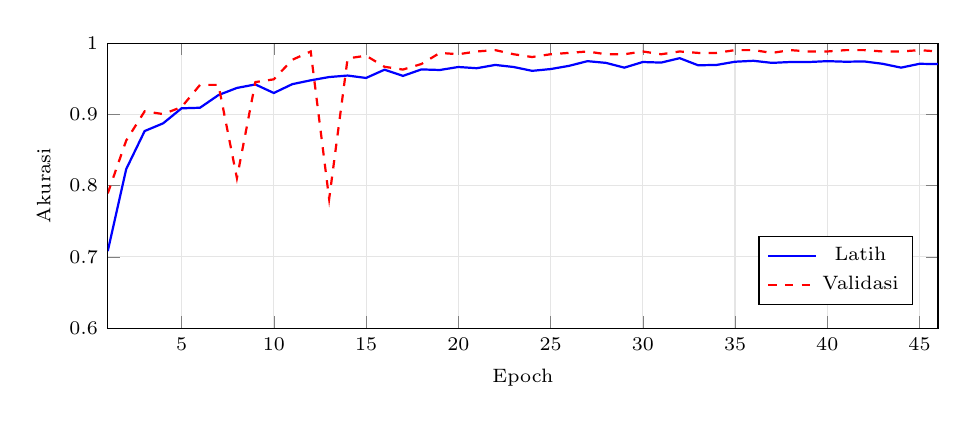
\begin{tikzpicture}
      \begin{axis}[
          width=\textwidth, height=5.2cm,
          xlabel={Epoch}, ylabel={Akurasi},
          font=\scriptsize, label style={font=\scriptsize},
          legend style={font=\scriptsize, at={(0.97,0.08)}, anchor=south east},
          ymin=0.6, ymax=1.0, xmin=1, xmax=46,
          grid=both, grid style={gray!20}
        ]
        \addplot[thick, blue] coordinates {
          (1,0.7081)(2,0.8232)(3,0.8766)(4,0.8874)(5,0.9085)(6,0.9093)(7,0.9271)
          (8,0.9371)(9,0.9420)(10,0.9300)(11,0.9424)(12,0.9478)(13,0.9524)(14,0.9545)
          (15,0.9511)(16,0.9627)(17,0.9540)(18,0.9631)(19,0.9623)(20,0.9665)(21,0.9648)
          (22,0.9694)(23,0.9665)(24,0.9611)(25,0.9636)(26,0.9681)(27,0.9747)(28,0.9723)
          (29,0.9656)(30,0.9735)(31,0.9727)(32,0.9789)(33,0.9689)(34,0.9694)(35,0.9739)
          (36,0.9752)(37,0.9723)(38,0.9735)(39,0.9735)(40,0.9747)(41,0.9739)(42,0.9743)
          (43,0.9710)(44,0.9656)(45,0.9710)(46,0.9706)
        };
        \addlegendentry{Latih}
        \addplot[thick, red, dashed] coordinates {
          (1,0.7891)(2,0.8633)(3,0.9043)(4,0.9004)(5,0.9102)(6,0.9414)(7,0.9414)
          (8,0.8105)(9,0.9453)(10,0.9492)(11,0.9766)(12,0.9883)(13,0.7812)(14,0.9785)
          (15,0.9824)(16,0.9668)(17,0.9629)(18,0.9707)(19,0.9863)(20,0.9844)(21,0.9883)
          (22,0.9902)(23,0.9844)(24,0.9805)(25,0.9844)(26,0.9863)(27,0.9883)(28,0.9844)
          (29,0.9844)(30,0.9883)(31,0.9844)(32,0.9883)(33,0.9863)(34,0.9863)(35,0.9902)
          (36,0.9902)(37,0.9863)(38,0.9902)(39,0.9883)(40,0.9883)(41,0.9902)(42,0.9902)
          (43,0.9883)(44,0.9883)(45,0.9902)(46,0.9883)
        };
        \addlegendentry{Validasi}
      \end{axis}
    \end{tikzpicture}
    {\small (a) Kurva akurasi}
  \end{minipage}
  \hfill
  \begin{minipage}{0.48\textwidth}
    \centering
    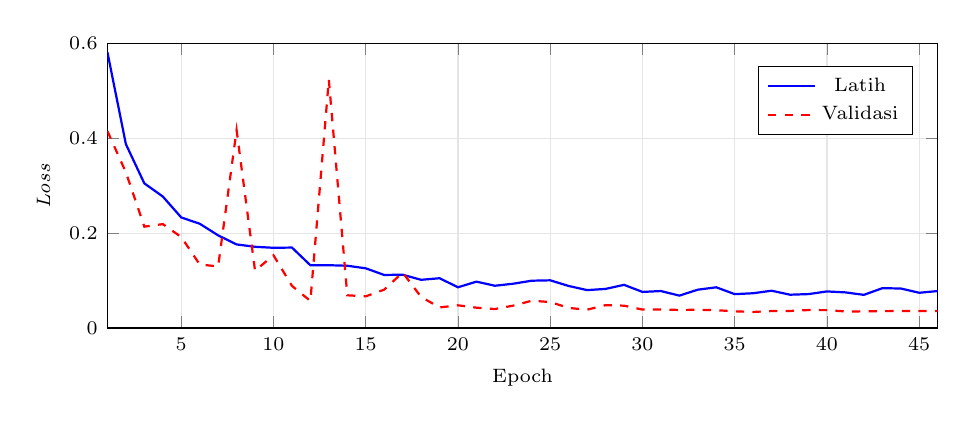
\begin{tikzpicture}
      \begin{axis}[
          width=\textwidth, height=5.2cm,
          xlabel={Epoch}, ylabel={\textit{Loss}},
          font=\scriptsize, label style={font=\scriptsize},
          legend style={font=\scriptsize, at={(0.97,0.92)}, anchor=north east},
          ymin=0, ymax=0.6, xmin=1, xmax=46,
          grid=both, grid style={gray!20}
        ]
        \addplot[thick, blue] coordinates {
          (1,0.5808)(2,0.3872)(3,0.3047)(4,0.2770)(5,0.2329)(6,0.2197)(7,0.1952)
          (8,0.1761)(9,0.1711)(10,0.1690)(11,0.1695)(12,0.1322)(13,0.1323)(14,0.1312)
          (15,0.1258)(16,0.1118)(17,0.1123)(18,0.1016)(19,0.1049)(20,0.0859)(21,0.0977)
          (22,0.0891)(23,0.0934)(24,0.0997)(25,0.1005)(26,0.0886)(27,0.0799)(28,0.0824)
          (29,0.0910)(30,0.0761)(31,0.0779)(32,0.0683)(33,0.0808)(34,0.0858)(35,0.0714)
          (36,0.0733)(37,0.0786)(38,0.0702)(39,0.0715)(40,0.0771)(41,0.0751)(42,0.0699)
          (43,0.0839)(44,0.0833)(45,0.0743)(46,0.0779)
        };
        \addlegendentry{Latih}
        \addplot[thick, red, dashed] coordinates {
          (1,0.4147)(2,0.3279)(3,0.2135)(4,0.2189)(5,0.1917)(6,0.1340)(7,0.1297)
          (8,0.4169)(9,0.1207)(10,0.1532)(11,0.0889)(12,0.0570)(13,0.5228)(14,0.0690)
          (15,0.0667)(16,0.0809)(17,0.1170)(18,0.0656)(19,0.0434)(20,0.0479)(21,0.0429)
          (22,0.0400)(23,0.0473)(24,0.0575)(25,0.0548)(26,0.0423)(27,0.0387)(28,0.0482)
          (29,0.0471)(30,0.0389)(31,0.0391)(32,0.0381)(33,0.0385)(34,0.0376)(35,0.0352)
          (36,0.0339)(37,0.0358)(38,0.0360)(39,0.0379)(40,0.0377)(41,0.0350)(42,0.0351)
          (43,0.0356)(44,0.0358)(45,0.0357)(46,0.0358)
        };
        \addlegendentry{Validasi}
      \end{axis}
    \end{tikzpicture}
    {\small (b) Kurva \textit{loss}}
  \end{minipage}
  \caption{Kurva Akurasi dan \textit{Loss} Selama Pelatihan Model CNN ADADeH (46 Epoch)}
  \label{fig:kurva-pelatihan}
\end{figure}

Gambar \ref{fig:kurva-pelatihan} memperlihatkan dua hal yang relevan dengan
keputusan desain. Pertama, \textit{validation loss} sempat melonjak tajam pada
beberapa epoch (misalnya epoch ke-8 dan ke-13) sebelum kembali turun, yang
merupakan pola umum pada pelatihan dengan \textit{learning rate} yang belum
diturunkan serta augmentasi SpecAugment yang membuat setiap \textit{batch}
pelatihan sedikit berbeda. Kedua, sejak \textit{learning rate} mulai diturunkan
(epoch ke-16 dan seterusnya), kurva validasi menjadi jauh lebih stabil, menunjukkan
bahwa \texttt{ReduceLROnPlateau} berperan penting dalam mencapai konvergensi yang
stabil pada model berukuran ringan ini.

\subsection{Implementasi Evaluasi Model}
\label{subsec:implementasi-evaluasi}

Evaluasi dilakukan dalam dua tahap sesuai KF-07: pencarian ambang keputusan $\tau$
pada data validasi, kemudian pengukuran kinerja pada data uji baik pada tingkat
potongan maupun tingkat berkas (hasil agregasi, Persamaan III.2).

\begin{lstlisting}[language=Python, caption={Pencarian ambang keputusan dan evaluasi model}, label={lst:evaluasi}]
pv = model.predict(X_val)[:, 1]
ths = np.linspace(0.05, 0.95, 91)
best_t = ths[np.argmax([f1_score(y_val, pv > t, average="macro") for t in ths])]

pt = model.predict(X_test)[:, 1]
pred = (pt > best_t).astype(int)

fid = test["file_id"]
files = np.unique(fid)
p_file = np.array([pt[fid == f].mean() for f in files])     # Persamaan III.2
y_file = np.array([y_test[fid == f][0] for f in files])
pred_file = (p_file > best_t).astype(int)
\end{lstlisting}

Pencarian pada 91 nilai ambang antara 0,05 dan 0,95 menghasilkan $\tau=0{,}51$
sebagai ambang yang memaksimalkan F1 makro pada data validasi. Nilai inilah yang
disimpan pada \texttt{meta.json} (Tabel \ref{tab:meta-json}) dan digunakan pada
Persamaan II.4 saat purwarupa menentukan label akhir. Perhitungan \texttt{p\_file}
pada baris ke-8 kode di atas secara langsung mengimplementasikan Persamaan III.2,
yaitu merata-ratakan skor seluruh potongan suatu berkas (diidentifikasi melalui
\texttt{file\_id}) menjadi satu skor berkas $\bar{p}$.

Tabel \ref{tab:evaluasi-chunk} dan \ref{tab:evaluasi-file} menyajikan hasil evaluasi
pada data uji untuk masing-masing tingkat.

\begin{table}[htbp]
  \centering
  \caption{Hasil Evaluasi pada Data Uji -- Tingkat Potongan ($n=507$)}
  \label{tab:evaluasi-chunk}
  \begin{tabular}{@{}lrrrr@{}}
    \toprule
    \textbf{Kelas} & \textbf{Presisi} & \textbf{\textit{Recall}} & \textbf{F1} & \textbf{Dukungan} \\
    \midrule
    \textit{Real} (asli) & $1{,}00$ & $0{,}98$ & $0{,}99$ & 305 \\
    \textit{Fake} (deepfake) & $0{,}97$ & $1{,}00$ & $0{,}99$ & 202 \\
    \midrule
    Akurasi keseluruhan & \multicolumn{4}{l}{$0{,}99$} \\
    ROC-AUC & \multicolumn{4}{l}{$0{,}9987$} \\
    EER & \multicolumn{4}{l}{$0{,}99\%$} \\
    \bottomrule
  \end{tabular}

  \vspace{2mm}
  \small Matriks konfusi (baris: label asli; kolom: label prediksi; urutan \textit{real}, \textit{fake}):
  $\begin{pmatrix} 299 & 6 \\ 0 & 202 \end{pmatrix}$
\end{table}

\begin{table}[htbp]
  \centering
  \caption{Hasil Evaluasi pada Data Uji -- Tingkat Berkas ($n=280$, Agregasi Persamaan III.2)}
  \label{tab:evaluasi-file}
  \begin{tabular}{@{}lrrrr@{}}
    \toprule
    \textbf{Kelas} & \textbf{Presisi} & \textbf{\textit{Recall}} & \textbf{F1} & \textbf{Dukungan} \\
    \midrule
    \textit{Real} (asli) & $1{,}00$ & $0{,}97$ & $0{,}99$ & 140 \\
    \textit{Fake} (deepfake) & $0{,}97$ & $1{,}00$ & $0{,}99$ & 140 \\
    \midrule
    Akurasi keseluruhan & \multicolumn{4}{l}{$0{,}99$} \\
    ROC-AUC & \multicolumn{4}{l}{$0{,}9971$} \\
    EER & \multicolumn{4}{l}{$1{,}43\%$} \\
    \bottomrule
  \end{tabular}

  \vspace{2mm}
  \small Matriks konfusi (baris: label asli; kolom: label prediksi; urutan \textit{real}, \textit{fake}):
  $\begin{pmatrix} 136 & 4 \\ 0 & 140 \end{pmatrix}$
\end{table}

Dibandingkan dengan kriteria keberhasilan pada Bab I (akurasi dan F1 minimal
$90\%$), hasil pada Tabel \ref{tab:evaluasi-chunk} dan \ref{tab:evaluasi-file}
menunjukkan pencapaian yang jauh melampaui target tersebut, baik pada tingkat
potongan maupun tingkat berkas. Nilai ROC-AUC yang sangat tinggi ($0{,}9987$ pada
tingkat potongan dan $0{,}9971$ pada tingkat berkas) juga mengindikasikan bahwa
kedua kelas dapat dipisahkan dengan sangat baik pada hampir seluruh nilai ambang.
Baris EER pada kedua tabel mengonfirmasi hal tersebut secara langsung: pada
notebook pengembangan, EER belum dihitung secara eksplisit, sehingga nilai pada
Tabel \ref{tab:evaluasi-chunk} dan \ref{tab:evaluasi-file} diperoleh kemudian
melalui modul \texttt{evaluation.py} pada aplikasi (dibahas pada Subsubbab
\ref{subsec:implementasi-evaluasi-app}), yang menghitung EER melalui interpolasi
linear pada kurva ROC sesuai Persamaan II.7, yaitu titik potong ketika
\textit{false positive rate} sama dengan \textit{false negative rate}. EER sebesar
$0{,}99\%$ pada tingkat potongan dan $1{,}43\%$ pada tingkat berkas menunjukkan
bahwa kesalahan klasifikasi hanya terjadi pada sebagian kecil dari seratus
rekaman, konsisten dengan cara verifikasi KNF-01 pada Tabel III.8.

Matriks konfusi pada kedua tabel juga menunjukkan pola yang konsisten: tidak ada
rekaman deepfake yang salah diklasifikasikan sebagai asli (\textit{false negative}
nol) pada kedua tingkat evaluasi, sedangkan sejumlah kecil rekaman asli
diklasifikasikan sebagai deepfake (6 potongan dan 4 berkas). Dari sisi tujuan
ADADeH untuk memberi indikasi awal bagi korban (Bab I), pola kesalahan seperti ini
relatif lebih aman dibandingkan sebaliknya, karena model pada tahap pengujian ini
cenderung lebih waspada terhadap deepfake daripada meloloskannya sebagai suara
asli.

\subsection{Implementasi Penyimpanan Artefak Model}
\label{subsec:implementasi-penyimpanan}

Setelah pelatihan dan evaluasi selesai, model, riwayat pelatihan, dan konfigurasi
disimpan sebagai tiga berkas terpisah agar dapat dimuat kembali oleh purwarupa
(Subbab \ref{subsec:arsitektur-konfigurasi}):

\begin{lstlisting}[language=Python, caption={Penyimpanan model dan konfigurasi}, label={lst:simpan-model}]
model.save(out + "adadeh_cnn.keras")

with open(out + "history.json", "w") as f:
    json.dump({k: [float(v) for v in vals] for k, vals in history.history.items()}, f)

meta = {
    "mu": float(mu), "sd": float(sd), "threshold": float(best_t),
    "global_sr": int(global_sr), "chunk_dur": int(chunk_dur), "step": int(step),
    "n_fft": 1024, "hop_length": 256, "n_mels": 128, "classes": classes,
}
with open(out + "meta.json", "w") as f:
    json.dump(meta, f)
\end{lstlisting}

Berkas \texttt{adadeh\_cnn.keras} (sekitar 1,4 MB) menyimpan arsitektur dan bobot
model secara utuh, \texttt{history.json} menyimpan riwayat metrik setiap epoch
untuk keperluan dokumentasi dan analisis lanjutan (termasuk Gambar
\ref{fig:kurva-pelatihan}), dan \texttt{meta.json} menyimpan seluruh parameter yang
telah dibahas pada Tabel \ref{tab:meta-json}. Ketiga berkas inilah yang kemudian
disertakan sebagai artefak aplikasi dan dimuat oleh modul inferensi pada
arsitektur klien--server (Subbab \ref{subsec:arsitektur-klien-server}). Subsubbab
berikut menjelaskan bagaimana artefak ini diintegrasikan ke dalam aplikasi
Streamlit yang telah dibangun, mulai dari validasi audio hingga pengujian
perangkat lunak.

\subsection{Implementasi Validasi dan Keamanan Audio}
\label{subsec:implementasi-audio}

Berbeda dengan notebook pengembangan yang membaca berkas dari dataset yang telah
terpercaya, aplikasi harus menerima unggahan dari pengguna mana pun, sehingga
modul \texttt{audio.py} dirancang dengan asumsi bahwa setiap berkas masukan
dapat berisi data yang keliru atau berbahaya. Validasi dijalankan berlapis
sebelum satu \textit{sample} audio pun diproses lebih jauh:

\begin{enumerate}
  \item \textbf{Pemeriksaan amplop berkas.} Ukuran dan beberapa \textit{byte}
  awal berkas diperiksa untuk memastikan jenis berkas sesuai dengan yang
  diklaim, sebelum berkas dibuka oleh pustaka dekode mana pun.
  \item \textbf{Pengerasan khusus untuk M4A/ISO-BMFF.} Berkas dengan wadah
  ISO-BMFF (termasuk M4A) diurai secara manual pada tingkat \textit{atom}
  untuk menolak berkas yang merujuk data pada lokasi eksternal (\textit{external
  data reference}), suatu teknik yang dapat dipakai untuk membaca berkas lain
  di luar yang diunggah pengguna.
  \item \textbf{Pemeriksaan melalui \texttt{ffprobe}.} Metadata audio (durasi,
  jumlah kanal, \textit{sampling rate}) diperiksa melalui \texttt{ffprobe}
  sebelum dekode penuh dijalankan, sehingga berkas yang jelas tidak valid dapat
  ditolak lebih awal (KF-02).
  \item \textbf{Dekode terisolasi proses.} Dekode audio sesungguhnya (melalui
  TorchCodec) dijalankan pada \textit{subprocess} terpisah dengan batas waktu 45
  detik dan batas sumber daya (memori dan CPU), sehingga berkas yang dirancang
  untuk menyebabkan dekoder mengonsumsi sumber daya tak terbatas
  (\textit{denial-of-service}) tidak dapat memengaruhi proses utama aplikasi
  (KNF-03, KNF-06).
\end{enumerate}

Keempat lapis ini menjalankan Tahap 1 pada Gambar \ref{fig:alur-proses} secara
lebih ketat dibandingkan asumsi awal pada Bab III, yang hanya menyebutkan
validasi ukuran dan durasi berkas. Penguatan ini diambil karena purwarupa pada
Bab III dan IV versi notebook belum memperhitungkan bahwa aplikasi akan
diakses secara langsung oleh pengguna yang tidak dikenal, sehingga permukaan
serangan (\textit{attack surface}) perlu dipersempit sebelum aplikasi
dipertimbangkan untuk diakses publik (lihat pembatasan pada Subbab
\ref{sec:rangkuman-bab-iv}).

\subsection{Implementasi Runtime Model dan Verifikasi Integritas}
\label{subsec:implementasi-model-runtime}

Modul \texttt{contracts.py} mendefinisikan \texttt{ModelContract} sebagai
\textit{frozen dataclass} yang memuat seluruh kunci pada Tabel
\ref{tab:meta-json}, beserta metode \texttt{normalize()} yang mengonversi nilai
JSON mentah (misalnya \textit{string} atau \textit{integer}) menjadi tipe data
Python yang konsisten dengan yang dipakai pada notebook (\textit{float} untuk
\texttt{mu}/\texttt{sd}/\texttt{threshold}, \textit{int} untuk parameter
pemotongan dan STFT). Kontrak ini kemudian dipakai oleh \texttt{model.py} pada
kelas \texttt{ModelRuntime}, yang bertanggung jawab atas tiga hal:

\begin{itemize}
  \item \textbf{Verifikasi integritas artefak.} Sebagaimana dijelaskan pada
  Subsubbab \ref{subsec:arsitektur-konfigurasi}, \textit{hash} SHA-256 berkas
  model dan konfigurasi dihitung saat pemuatan dan dibandingkan dengan konstanta
  \texttt{MODEL\_SHA256} dan \texttt{META\_SHA256} yang tertanam pada kode;
  ketidaksesuaian menghentikan pemuatan tanpa cadangan otomatis.
  \item \textbf{Pendaftaran ulang lapisan khusus.} Karena model memakai lapisan
  \texttt{SpecAugment} buatan sendiri (Kode Program \ref{lst:specaugment}),
  modul ini mendaftarkan kembali lapisan tersebut sebagai \textit{custom object}
  Keras agar \texttt{adadeh\_cnn.keras} dapat dimuat ulang tanpa kesalahan
  \textit{deserialization}.
  \item \textbf{Validasi bentuk masukan secara ketat.} Sebelum memanggil
  \texttt{model.predict}, bentuk larik masukan diperiksa agar persis
  $(\cdot,128,157,1)$ sesuai Tabel \ref{tab:lapisan-cnn}; ketidaksesuaian bentuk
  menimbulkan kesalahan eksplisit alih-alih dibiarkan menghasilkan keluaran yang
  salah secara diam-diam, sejalan dengan prinsip konsistensi parameter pada
  Subsubbab \ref{subsec:prinsip-desain}.
\end{itemize}

Inferensi dijalankan dalam mode \textit{batch} dengan penguncian
(\textit{thread lock}), sehingga pemanggilan model dari beberapa permintaan
pengguna secara bersamaan tidak saling bertabrakan pada objek model Keras yang
sama (KNF-06). Label akhir dan skor keyakinan kemudian ditentukan oleh
\texttt{prediction.py} melalui fungsi \texttt{classify\_scores()}, yang
menerapkan operator ambang ketat lebih besar ($\bar{p} > \tau$), persis seperti
pencarian ambang pada Kode Program \ref{lst:evaluasi}, dan menghasilkan label
teks ``Terindikasi deepfake'' atau ``Terindikasi asli'' sesuai rancangan pada
Tabel \ref{tab:elemen-keluaran}.

\subsection{Implementasi Pemeriksaan Mutu Rekaman}
\label{subsec:implementasi-mutu}

Modul \texttt{quality.py} mengimplementasikan \texttt{QualityPolicy}, yaitu
kebijakan ambang tetap yang menjadi dasar peringatan mutu pada Tabel
\ref{tab:elemen-keluaran} (KF-10, KP-07). Fungsi \texttt{assess\_quality()}
memeriksa empat kondisi atas rekaman yang telah lolos validasi pada Subsubbab
\ref{subsec:implementasi-audio}, dirangkum pada Tabel \ref{tab:kebijakan-mutu}.

\begin{table}[htbp]
  \centering
  \caption{Kebijakan Pemeriksaan Mutu Rekaman (\texttt{QualityPolicy})}
  \label{tab:kebijakan-mutu}
  \begin{tabular}{@{}lp{8.6cm}@{}}
    \toprule
    \textbf{Kondisi} & \textbf{Ambang} \\
    \midrule
    Hening (\textit{silence}) & Sedikitnya $90\%$ bingkai berada di bawah $-50$ dBFS \\
    Level rendah & Level keseluruhan rekaman di bawah $-35$ dBFS \\
    \textit{Clipping} & Sedikitnya $1\%$ sampel mencapai amplitudo $\geq 0{,}999$ \\
    Durasi singkat & Durasi rekaman kurang dari $3{,}75$ detik \\
    \bottomrule
  \end{tabular}
\end{table}

Keempat kondisi ini bersifat tidak saling meniadakan (satu rekaman dapat
memenuhi lebih dari satu kondisi) dan tidak menggagalkan proses deteksi;
peringatan yang dihasilkan hanya ditambahkan pada elemen keluaran ``Peringatan
mutu'' (Tabel \ref{tab:elemen-keluaran}) agar pengguna memahami konteks hasil,
sejalan dengan prinsip pada Subsubbab \ref{subsec:alur-proses-sistem} bahwa
rekaman bermutu rendah tetap diproses, bukan ditolak.

\subsection{Implementasi Layanan, Antarmuka, dan Pelaporan}
\label{subsec:implementasi-layanan}

Modul \texttt{service.py} mengikat seluruh modul pada Subsubbab
\ref{subsec:implementasi-audio} sampai \ref{subsec:implementasi-mutu} menjadi
satu fungsi orkestrasi \texttt{analyze\_audio()}, yang dipanggil oleh antarmuka
pada \texttt{ui.py} setiap kali pengguna mengunggah rekaman. Fungsi ini
menjalankan Tahap 1 sampai 7 pada Gambar \ref{fig:alur-proses} secara berurutan
dan mengembalikan satu struktur hasil yang memuat label, skor, peringatan mutu,
dan metadata yang diperlukan untuk pelaporan.

Antarmuka pengguna dibangun dengan Streamlit (\texttt{ui.py},
\texttt{streamlit\_app.py} sebagai titik masuk) sesuai rancangan keluaran pada
Tabel \ref{tab:elemen-keluaran}. Dua keputusan implementasi berikut relevan
dengan prinsip desain pada Subsubbab \ref{subsec:prinsip-desain}:

\begin{itemize}
  \item \textbf{Pemuatan model satu kali.} Fungsi pemuat model didekorasi dengan
  \texttt{@st.cache\_resource} sehingga \texttt{ModelRuntime} (Subsubbab
  \ref{subsec:implementasi-model-runtime}) hanya dimuat dan diverifikasi
  integritasnya sekali per siklus hidup proses server, bukan setiap kali
  pengguna mengunggah rekaman -- memenuhi pertimbangan efisiensi sumber daya
  pada Subbab II.3.1.
  \item \textbf{Penanganan kesalahan yang menjaga privasi.} Pesan kesalahan yang
  ditampilkan kepada pengguna (misalnya saat validasi audio gagal) ditulis
  secara umum dan tidak menyertakan jejak kesalahan (\textit{stack trace}) atau
  nama berkas asli, sejalan dengan prinsip pemisahan tanggung jawab klien dan
  server pada Subsubbab \ref{subsec:prinsip-desain} serta KNF-05.
\end{itemize}

Setelah hasil ditampilkan, modul \texttt{reporting.py} menyediakan dua fungsi
pembangkit ringkasan terunduh sesuai Tabel \ref{tab:elemen-keluaran}:
\texttt{to\_json()} menghasilkan berkas JSON terstruktur (nama berkas, durasi,
waktu pemeriksaan, \textit{hash} SHA-256 rekaman, label, skor, versi model, dan
keterangan batasan), sedangkan \texttt{to\_text()} menghasilkan ringkasan yang
sama dalam bentuk teks naratif yang dapat dibaca langsung oleh pendamping
pelaporan (KF-11, KP-09). Sejalan dengan KF-12 dan KNF-05, baik berkas unggahan
maupun data antara (waveform dan mel-spectrogram sementara) tidak pernah
dituliskan ke penyimpanan permanen di luar sesi pemrosesan yang sedang
berjalan.

\subsection{Implementasi Evaluasi Purwarupa dan Reproduksi \textit{Baseline}}
\label{subsec:implementasi-evaluasi-app}

Untuk memastikan bahwa artefak model yang disertakan pada aplikasi benar-benar
identik perilakunya dengan model yang dilatih pada notebook (KNF-08), modul
\texttt{evaluation.py} menyediakan dua fungsi. Fungsi \texttt{binary\_metrics()}
menghitung akurasi, presisi/\textit{recall}/F1, matriks konfusi, ROC-AUC, dan
EER atas sepasang label dan skor, sedangkan \texttt{evaluate\_artifacts()}
memuat ulang \texttt{test.npz} serta model dan konfigurasi tersimpan, menjalankan
inferensi, lalu membandingkan matriks konfusi dan ROC-AUC yang dihasilkan
terhadap nilai acuan yang diambil langsung dari notebook (Tabel
\ref{tab:evaluasi-chunk} dan \ref{tab:evaluasi-file}); perbedaan di luar
toleransi numerik yang kecil akan menggagalkan pemeriksaan ini, sehingga
pemeriksaan berfungsi sebagai uji reproduksi \textit{baseline}, bukan sekadar
evaluasi ulang. Skrip \texttt{scripts/evaluate\_model.py} menyediakan antarmuka
baris perintah bagi kedua fungsi tersebut.

EER dihitung melalui interpolasi linear pada kurva ROC (\textit{false positive
rate} terhadap \textit{false negative rate}) untuk mencari titik potong kedua
kurva tersebut, sesuai rumusan pada Persamaan II.7. Nilai inilah yang telah
disertakan pada baris EER Tabel \ref{tab:evaluasi-chunk} dan
\ref{tab:evaluasi-file} pada Subsubbab \ref{subsec:implementasi-evaluasi}: EER
sebesar $0{,}99\%$ pada tingkat potongan dan $1{,}43\%$ pada tingkat berkas.
Kedua nilai ini diperoleh dengan menjalankan ulang model dan data uji yang
identik dengan notebook, dan menghasilkan matriks konfusi serta ROC-AUC yang
sama persis dengan Tabel \ref{tab:evaluasi-chunk} dan \ref{tab:evaluasi-file},
sehingga EER dapat dianggap sebagai pelengkap metrik yang sudah ada tanpa
mengubah kesimpulan evaluasi sebelumnya.

\subsection{Pengujian Perangkat Lunak}
\label{subsec:implementasi-pengujian}

Mengikuti pemisahan tanggung jawab antarmodul pada Tabel
\ref{tab:modul-pemrosesan}, aplikasi disertai rangkaian pengujian otomatis
menggunakan \texttt{pytest} yang dikelompokkan melalui \textit{marker} menjadi
empat kategori, dirangkum pada Tabel \ref{tab:kategori-pengujian}.

\begin{table}[htbp]
  \centering
  \caption{Kategori Pengujian Otomatis Aplikasi ADADeH}
  \label{tab:kategori-pengujian}
  \begin{tabular}{@{}lp{8.8cm}@{}}
    \toprule
    \textbf{Kategori} & \textbf{Lingkup Pengujian} \\
    \midrule
    Unit & Menguji setiap fungsi modul (Tabel \ref{tab:modul-pemrosesan}) secara
    terisolasi, misalnya \texttt{assess\_quality()} dan \texttt{classify\_scores()} \\
    Kesetaraan (\textit{parity}) & Membandingkan keluaran fungsi pada paket
    \texttt{adadeh} terhadap fungsi setara pada notebook (misalnya
    \texttt{extract\_features} terhadap \texttt{gen\_melspec\_data}, Kode Program
    \ref{lst:gen-melspec}) agar tidak ada penyimpangan perilaku akibat penulisan
    ulang kode \\
    Integrasi & Menguji \texttt{analyze\_audio()} (\texttt{service.py}) secara
    menyeluruh, dari berkas audio masukan hingga hasil akhir \\
    Antarmuka (UI) & Menguji elemen antarmuka Streamlit pada \texttt{ui.py} \\
    \bottomrule
  \end{tabular}
\end{table}

Keberadaan kategori kesetaraan secara khusus menjadi bukti tambahan -- selain
reproduksi \textit{baseline} pada Subsubbab \ref{subsec:implementasi-evaluasi-app}
-- bahwa penyesuaian implementasi dari notebook ke paket \texttt{adadeh} (seperti
pemecahan \texttt{gen\_melspec\_data} menjadi \texttt{preprocessing.py} yang
dapat diuji terpisah) tidak secara tidak sengaja mengubah hasil pemrosesan audio
maupun keputusan model. Sejalan dengan README pengembangan aplikasi, status
pengujian ini merupakan \textit{checkpoint} pengembangan yang sudah mencakup
keempat kategori di atas, namun belum disertai satu kali jalur pengujian penuh
(\textit{full test suite}) dan pemeriksaan keamanan yang selesai tanpa kendala
waktu jalan (\textit{timeout}), sehingga belum diklaim sebagai rilis produksi
(lihat pembatasan pada Subbab \ref{sec:rangkuman-bab-iv}).

\section{Rangkuman}
\label{sec:rangkuman-bab-iv}

Bab ini telah menjabarkan desain sistem ADADeH yang menerjemahkan kebutuhan
fungsional dan nonfungsional pada Bab III menjadi alur proses dan rancangan
keluaran yang konkret (Subbab \ref{sec:desain-sistem}), arsitektur klien--server
beserta susunan paket perangkat lunak \texttt{adadeh} dan model CNN yang
menjalankannya (Subbab \ref{sec:arsitektur-sistem}), dan implementasi purwarupa
yang telah dikerjakan secara lengkap, mulai dari akuisisi data dan pelatihan
model pada notebook hingga aplikasi Streamlit yang telah dibangun dan dapat
dijalankan pengguna (Subbab \ref{sec:implementasi}). Model CNN yang dihasilkan
mencapai akurasi dan F1 di atas $99\%$ pada data uji, melampaui target minimal
$90\%$ pada Bab I, dengan model yang ringan (sekitar 110 ribu parameter) sesuai
pertimbangan sumber daya pada Subbab III.3; EER yang dihitung kemudian melalui
modul evaluasi aplikasi (Subsubbab \ref{subsec:implementasi-evaluasi-app})
sebesar $0{,}99\%$ pada tingkat potongan dan $1{,}43\%$ pada tingkat berkas
memperkuat kesimpulan bahwa kedua kelas dapat dipisahkan dengan sangat baik.

Antarmuka Streamlit beserta integrasinya dengan modul inferensi -- yang pada
versi sebelumnya bab ini masih berstatus belum diimplementasikan -- telah
dibangun secara nyata sebagai paket Python \texttt{adadeh} (Subbab
\ref{subsec:arsitektur-modul-pemrosesan}) lengkap dengan validasi dan pengerasan
keamanan audio, verifikasi integritas artefak model, pemeriksaan mutu rekaman,
serta pelaporan hasil yang dapat diunduh (Subsubbab
\ref{subsec:implementasi-audio} sampai \ref{subsec:implementasi-pengujian}).
Meskipun demikian, sejalan dengan dokumentasi pengembangan aplikasi, purwarupa
ini tetap berstatus \textit{checkpoint} pengembangan dan bukan rilis produksi,
dengan sejumlah pembatasan yang menjadi acuan pekerjaan pada Bab V:

\begin{itemize}
  \item Masukan hanya berupa unggahan satu berkas melalui peramban; perekaman
  langsung melalui mikrofon belum tersedia.
  \item Analisis hanya mencakup maksimum $K{=}4$ potongan pertama (sekitar
  6,25 detik pertama rekaman); rekaman yang lebih panjang belum dianalisis
  secara menyeluruh, dan aplikasi menampilkan peringatan eksplisit mengenai
  keterbatasan cakupan ini kepada pengguna.
  \item Risiko penggunaan memori berlebih (\textit{out-of-memory}) pada proses
  \textit{resampling} untuk \textit{sampling rate} masukan yang tidak umum
  belum terselesaikan, sehingga aplikasi belum direkomendasikan untuk diakses
  publik atau menerima unggahan dari sumber yang tidak dipercaya tanpa
  pengawasan tambahan.
  \item Pengujian otomatis pada peramban (Tabel \ref{tab:kategori-pengujian},
  kategori UI) belum selesai secara menyeluruh, dan satu kali jalur pengujian
  penuh beserta pemeriksaan keamanan belum berhasil diselesaikan tanpa
  \textit{timeout}, sehingga belum dapat diklaim sebagai hasil pengujian yang
  bersih secara penuh.
\end{itemize}

Keempat pembatasan di atas bersifat jujur dan dapat ditindaklanjuti, bukan
kegagalan desain: keempatnya berasal dari keputusan sadar untuk membatasi
cakupan purwarupa demi keamanan dan kesederhanaan implementasi pada tahap ini,
sejalan dengan sifat iteratif pendekatan CRISP-DM pada Bab I.